\documentclass[12p,a4paper]{article}
\usepackage[utf8]{inputenc}
\usepackage[T1]{fontenc,url}
\usepackage{multicol}
\usepackage{multirow}
\usepackage{parskip}
\usepackage{lmodern}
\usepackage{microtype}
\usepackage{verbatim}
\usepackage{amsmath, amssymb}
\usepackage{tikz}
\usepackage{physics}
\usepackage{mathtools}
\usepackage{algorithm}
\usepackage{algpseudocode}
\usepackage{listings}
\usepackage{enumerate}
\usepackage{graphicx}
\usepackage{float}
\usepackage{hyperref}
\usepackage{tabularx}
\usepackage{siunitx}
\usepackage{fancyvrb}
\usepackage[makeroom]{cancel}
\usepackage[margin=2.0cm]{geometry}
\renewcommand{\baselinestretch}{1}
\renewcommand{\exp}{e^}
\renewcommand{\b}{\boldsymbol}
\newcommand{\h}{\hat}
\newcommand{\m}{\mathbb}
\newcommand{\half}{\frac{1}{2}}
\renewcommand{\exp}{e^}
\renewcommand{\bar}{\overline}
\setlength\parindent{0pt}


\begin{document}
\title{PHYSICS 141A -- Problem Set 1}
\author{
    \begin{tabular}{r l}
        Jonas Gahr Sturtzel Lunde & (\texttt{jonassl})
    \end{tabular}}
% \date{}    % if commented out, the date is set to the current date

\maketitle

\hspace{10cm}

\section*{Exercise 1}
\subsection*{a)}
\subsubsection*{$\rhd$}
\[
    Z = \int \frac{\dd{\b p}}{(2\pi\hbar)^3}\int \dd{\b x} \exp{-\beta H(\b p, \b x)}
\]
Classically, the momentum and position can take any value, so the integral limits are $\pm \infty$. Also, since $\b p$ and $\b x$ are vectors, this is the product of three identical intragrals, giving
\[
    Z = \qty[\frac{1}{2\pi\hbar}\int_{-\infty}^{\infty} \dd{\b p} \int_{-\infty}^{\infty} \dd{\b x} \exp{-\beta H(\b p, \b x)}]^3 = \qty[Z_{1D}]^3
\]
where
\[
    Z_{1D} = \frac{1}{2\pi\hbar}\int_{-\infty}^{\infty} \dd{ p} \int_{-\infty}^{\infty} \dd{ x} \exp{-\beta p^2 /2m }\exp{-\beta x^2k/2} = \frac{1}{2\pi\hbar}\int_{-\infty}^{\infty} \dd{p} \exp{-\beta p^2 /2m } \int_{-\infty}^{\infty} \dd{ x}\exp{-\beta x^2k/2}
\]
which is the product of two integrals on the known solution form
\[
    \int_{-\infty}^{\infty} \exp{-\lambda x^2} = \sqrt{\frac{\pi}{\lambda}}
\]
giving
\[
    Z_{1D} = \frac{1}{2\pi\hbar}\cdot \sqrt{\frac{2\pi m}{\beta}}\cdot \sqrt{\frac{2\pi}{\beta\hbar}} = \sqrt{\frac{m}{k\beta^2\hbar^2}} = \frac{1}{\beta\hbar\omega}
\]
such that the 3D partition function becomes
\[
    Z = [Z_{1D}]^3 = \qty(\frac{1}{\beta\hbar\omega})^3 = \qty(\frac{k_BT}{\hbar\omega})^3
\]


\subsubsection*{$\rhd$}
To derive the heat capacity, we require the average energy. Luckily, this can be derived from the partition function as
\[
    \langle E \rangle -\frac{1}{Z}\pdv{Z}{\beta} = -(\beta\hbar\omega)^3 \cdot\qty(-3\frac{1}{\beta^4\hbar^3\omega^3}) = \frac{3}{\beta} = 3k_BT
\]
The heat capacity then becomes
\[
    C = \pdv{\langle E \rangle}{T} = 3k_B
\]
which we know as the heat capacity relation of Dulong and Petit.


\subsubsection*{$\rhd$}
We have already shown that the heat capacity of a single haromnic oscilator is $C = k_B$. If you consider a solid of $N$ particles in 3D harmonic oscilator wells, then each particle can be modelled as a 3 independent 1D harmonic oscilators, just as modelled in the last exercise. Since these are all independent, and heat capacity is an extensive property (double the system, double the heat capacity), we can simply multiply the head capacity in the last exercise by the number of particles:
\[
    C = 3k_BN = 3R
\]



\subsection*{b)}
\subsubsection*{$\rhd$}
As in the last exercise, the 3D partition function just becomes a product of the individual partition functions:
\[
    Z = \sum_j \exp{-\beta E_j} = \sum_{n_x,n_y,n_z = 0}^{\infty} \exp{-\beta \omega\hbar(n_x + n_y + n_z + 3/2)} = \qty[\sum_{n = 0}^{\infty} \exp{-\beta \omega\hbar(n + 1/2)}]^3 = [Z_{1D}]^3
\]
where, we have the geometric sum
\[
    \sum_{0}^\infty \exp{-c(n+1/2)} = \frac{\exp{c/2}}{\exp{c} - 1}
\]
giving the partition function
\[
    Z = \qty[\frac{\exp{-\beta\omega\hbar/2}}{\exp{-\beta\omega\hbar} - 1}]^3
\]



\subsubsection*{$\rhd$}
Bose statistics deals with the low energy occupancy of bosons, where any number of particles can occupy the same state. This can be modelled as above, with 3N independent harmonic oscilators. These calculations, unlike the ones in exercise a, works in the low temperature limit, where quantum mechanics rule, and energy levels are discrete. We will later see that the law appraches Dulong and Petit, and the classical picture, in the high temperature limit.



\subsubsection*{$\rhd$}
We will solve for the heat capacity in similiar fashion as exercise a, but this time we use the energy relation
\begin{align*}
    \langle E \rangle = -\pdv{\beta}\qty[\ln(Z)] = -3\pdv{\beta}\qty[\ln(\exp{-\beta\omega\hbar/2}) - \ln(\exp{-\beta\omega\hbar} - 1)] \\
    = 3\pdv{\beta}\beta\omega\hbar/2 + 3\pdv{\beta}\ln(\exp{-\beta\omega\hbar} - 1)
    = \frac{3}{2}\omega\hbar + \frac{3\omega\hbar}{\exp{\beta\omega\hbar} - 1}\\
    = 3\omega\hbar\qty[\frac{1}{\exp{\beta\omega\hbar} - 1} + \frac{1}{2}]
\end{align*}

The heat capacity then becomes
\[
C = \pdv{\langle E \rangle}{T} = \pdv{T}3\omega\hbar\qty[\frac{1}{\exp{\omega\hbar/k_BT} - 1} + \frac{1}{2}] = 3\omega\hbar\frac{\omega\hbar\exp{\omega\hbar/k_BT}}{k_BT^2\qty(\exp{\omega\hbar/k_BT} - 1)^2}
\]


\subsubsection*{$\rhd$}
In the high-temperature limit ($\beta \ll 1$), we can apply the first order expansion $\exp{\beta\omega\hbar} \approx 1 + \beta\omega\hbar$, giving

\[
    C = \frac{3\omega^2\hbar^2(1 + \omega\hbar/k_BT)}{k_BT^2\qty(1 + \omega\hbar/k_BT - 1)^2}
    = 3\frac{\omega^2\hbar^2}{\omega^2\hbar^2/k_B}(1 + \omega\hbar/k_BT) = 3(k_B + \frac{\omega\hbar}{T})
\]
which approaches $C = 3k_B$ for the $T \gg 1$ limit, in agreement with Dulong and Petit.


\subsubsection*{$\rhd$}
Scaled C vs T plot, sketched in Python.
\begin{figure}[H]
    \centering
    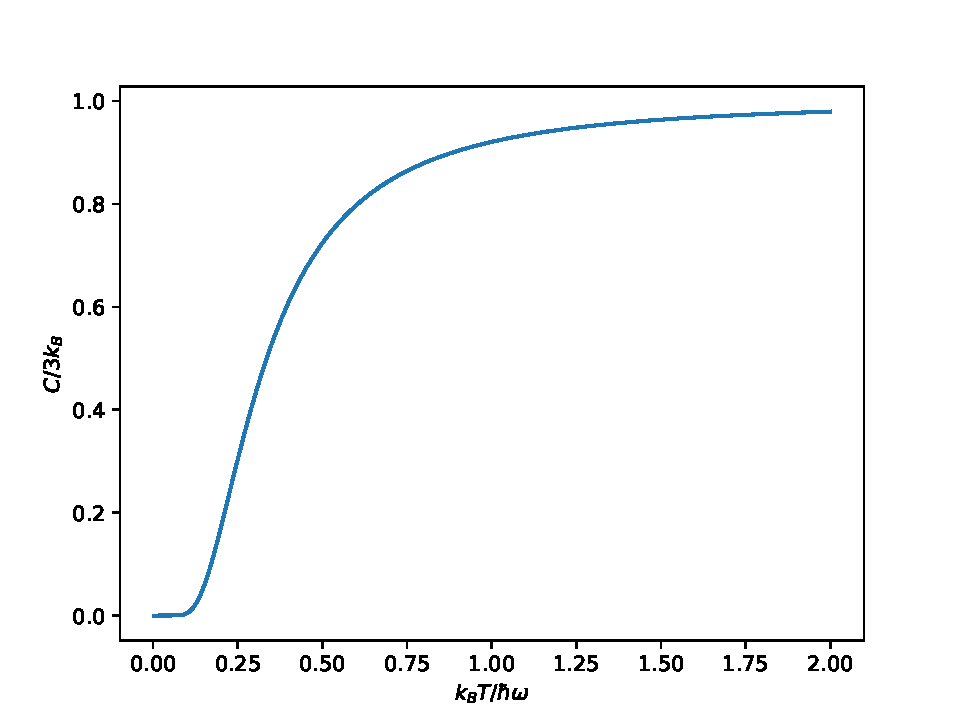
\includegraphics[width=0.6\linewidth]{asdf.pdf}
\end{figure}




\section*{Exercise 2}
With the given spring constant energy at the given distance, we can calculate $k$ to be
\[
    U = \frac{kx^2}{2} \quad\Rightarrow\quad
    \SI{1}{eV} = \frac{k \cdot \SI{1}{Å}^2}{2} \quad\Rightarrow\quad k = \SI{2}{eV/Å^2} = \SI{32.04}{J/m^2}
\]

For carbon, we get the oscilation frequency
\[
    \omega_c = \sqrt{\frac{k}{m_c}} = \sqrt{\frac{\SI{32.04}{J/m^2}}{12\times \SI{1.661e-27}{kg}}} = \SI{4.01e13}{s^{-1}}
\]

\[
    \omega_p = \sqrt{\frac{k}{m_c}} = \sqrt{\frac{\SI{32.04}{J/m^2}}{195\times \SI{1.661e-27}{kg}}} = \SI{9.95e12}{s^{-1}}
\]

The ration between their oscilation frequencies is
\[
    \frac{\omega_c}{\omega_p} = 4.03 \approx \sqrt{16.25} = \sqrt{\frac{m_p}{m_c}}
\]
Since the frequency goes as $m^{-1/2}$), we would expect the ratio of frequencies to go as the squareroot of the ratio of masses, as we can see that it does.

The corresponding temperatures become
\[
    T_c = \frac{\omega \hbar}{k_B} = \frac{\SI{4.01e13}{s^{-1}}\times \SI{1.0546e-34}{m^2kg/s}}{\SI{1.3806e-23}{m^2kg/s^2K}} = \SI{306.3}{K}
\]
\[
    T_p = \frac{\omega \hbar}{k_B} = \frac{\SI{9.95e12}{s^{-1}}\times \SI{1.0546e-34}{m^2kg/s}}{\SI{1.3806e-23}{m^2kg/s^2K}} = \SI{76}{K}
\]

For carbon, this is basically room temperature. $k=\SI{2}{eV/Å}$ is then probably a reasonable estimate on the bonding strength between carbons in a solid at room temperature. This did however assume a 1D harmonic oscilator, so these numbers might not apply to real solids.


\section*{Exercise 3}
The equation of motion (from N2L) for the electrons in a solid, under the influence of an electric field $E$, and under the influence of an average scattering time $\tau$, is as known
\[
    \dv{\b p}{t} = -e\b E - \frac{\b p}{\tau}
\]

Looking at a 1D problem, and introducing an oscilating electric field $E = E_0 \exp{i\omega t}$, we get the first order, linear differential equation
\[
    \dv{p}{t} = -eE_0 \exp{i\omega t} - \frac{p}{\tau}
\]
The oscilating electric field means we can not assume a steady-state solution, and are left with the general solutions
\[
    p(t) = c_1 \exp{-t/\tau} + eE_0\tau\frac{\exp{-i\omega t}}{i\omega \tau - 1}
\]
The first term holds whatever starting momentum the electrons might have had when turning on the electric field. As we can see, it would decay over time, and isn't really of much interest in this problem. We can simply assume the electrons start with some velocity which makes this term 0.

Throwing away the exponential term and inserting the momentum into the expression for current gives
\[
    j(t) = -\frac{enp}{m} = -\frac{e^2nE_0\tau}{m}\frac{\exp{-i\omega t}}{i \omega \tau - 1}
\]
which is just a harmonic oscilation in real and complex space.

The optical conductivity becomes
\[
    \sigma(\omega) = \frac{j(\omega)}{E(\omega)} = \frac{e^2n\tau}{(i\omega\tau - 1)m}
\]

\subsection*{Shit gets $\m R$eal}
The real part of the electric field is $\m R(E) = \m R\qty[E_0\cos(i\omega t) + i\sin(\omega t)] = E_0\cos(i\omega t)$.

Now, deriving the real part of the current can either be done by solving differential equation again with a real electric field, or, as we will do, multiply the equation by 1, disguied as the complex conjugate of our denominator, $\frac{1 + i\omega\tau}{1 + i\omega\tau}$, giving
\[
    j(t) = -\frac{e^2nE_0\tau}{m}(i\omega\tau + 1 )\frac{\exp{-i\omega t}}{1+\omega^2\tau^2} = -\frac{e^2nE_0\tau}{m}(i\omega\tau + 1 ) \frac{\cos(\omega t) + i\sin(\omega t)}{1 + \omega^2\tau^2}
\]
The surviving real parts of this product is
\[
    \m R[j(t)] = \frac{e^2nE_0\tau}{m}\qty(\frac{\cos(\omega t)}{1 + \omega^2\tau^2} + \frac{\omega\tau \sin(\omega t)}{1+\omega^2\tau^2})
\]

\subsection*{The Limit $\omega\tau \ll 1$}
For the limit $\omega\tau \ll 1$, we can assume that $(1 + \omega^2\tau^2) \approx 1$, giving
\[
    \m R(j(t)) \approx \frac{e^2nE_0\tau}{m}\qty(\cos(\omega t) + \omega\tau\sin(\omega t)) \approx \frac{e^2nE_0}{m}\cos(\omega t)
\]
as the $\omega\tau$ term in from of the sine will go to zero.

Looking back at the electric field, we notice that the current for this limit is in phase with electric field.

\subsection*{The Limit $\omega\tau \gg 1$}

For the limit $\omega\tau \gg 1$, we can instead assume that $(1 + \omega^2\tau^2) \approx \omega^2\tau^2$, instead giving
\[
    \m R(j(t)) \approx \frac{e^2nE_0\tau}{m}\qty(\frac{\cos(\omega t)}{\omega^2\tau^2} + \frac{\sin(\omega t)}{\omega \tau}) \approx \frac{e^2nE_0}{m\omega}\sin(\omega t)
\]
as the $1/(\omega\tau)$ term will dominate the $1/(\omega^2\tau^2)$ term.

For this limit, the current is completely out of phase with the electric field.

Both currents and the field is plotted below. They are all scaled to 1, as all have different units. The phase is what matters, and we see exactly what we described above.
\begin{figure}[H]
    \centering
    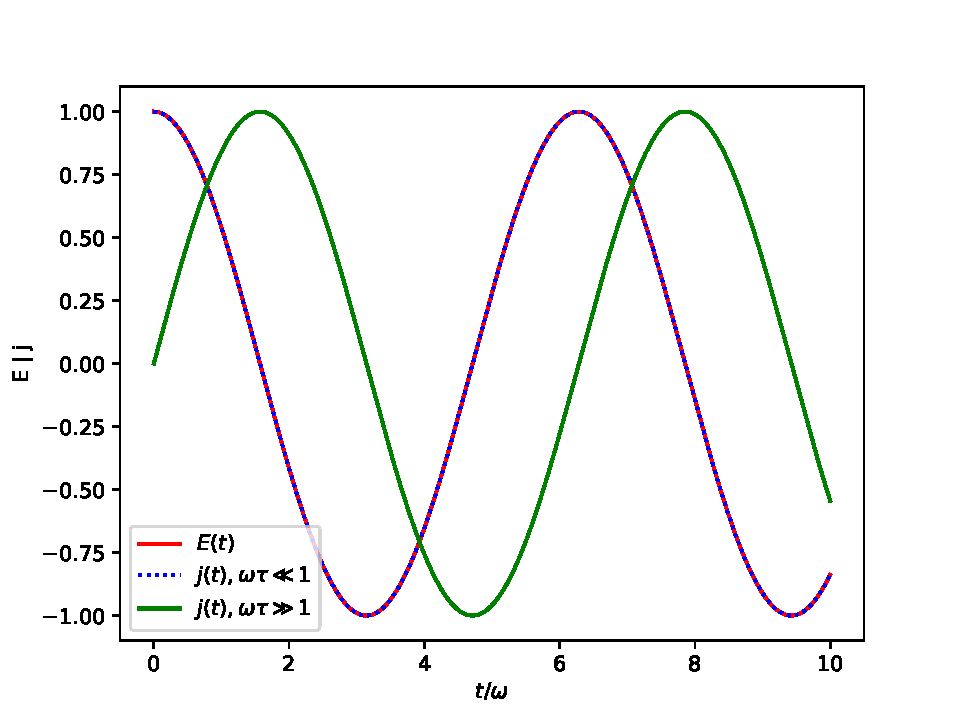
\includegraphics[width=0.6\linewidth]{asdf2.pdf}
\end{figure}


To conclude, if the electric oscilating frequency $\omega$, or the relaxation time $\tau$ gets too large, the current gets out of phase. A large oscilation frequency will leave the electrons unable to respond to the shift, due to their intertia. This, however, can be countermeasured by a reduction in $\theta$, which means the electrons will more often stop dead in their tracks, enabling them to change direction.

Note that these were the two extreme limits. In a compromise case, the current would be somewhere in between 0 and 90 degrees out of phase, depending on the size of $\omega\tau$.
\end{document}